% =============================================================================
% Week 5: Fixed Effects Regressions in Corporate Finance
% =============================================================================
\documentclass[aspectratio=169, 11pt]{beamer}

\usepackage{beamerthemeFixedEffects}
\usepackage{booktabs}
\usepackage{tikz}
\usetikzlibrary{positioning, arrows.meta, calc}
\usepackage{graphicx}
\usepackage{amsmath}
\usepackage{xcolor}
\usepackage{fancyvrb}

% ── Metadata ───────────────────────────────────────────────────────────────────
\title[Fixed Effects in Corporate Finance]{Fixed Effects Regressions\\in Corporate Finance}
\subtitle{Why specification choice determines what your coefficient means}
\author{Dissertation Module}
\institute{Week 5}
\date{}

\begin{document}

% ━━━━━━━━━━━━━━━━━━━━━━━━━━━━━━━━━━━━━━━━━━━━━━━━━━━━━━━━━━━━━━━━━━━━━━━━━━━━
\begin{frame}[plain]
  \titlepage
\end{frame}

% ━━━━━━━━━━━━━━━━━━━━━━━━━━━━━━━━━━━━━━━━━━━━━━━━━━━━━━━━━━━━━━━━━━━━━━━━━━━━
\section{The Problem}

% ──────────────────────────────────────────────────────────────────────────────
\begin{frame}{Pooled OLS overstates the patent--innovation relationship by 38\%}

\vspace{0.4cm}
\begin{columns}[T]
\begin{column}{0.52\textwidth}

A naive regression of process innovation on patent stock yields
$\hat{\beta} = 0.847$.

\vspace{0.5cm}

But this estimate confounds the \alert{within-firm} effect
(does a firm innovate more when its patent stock grows?)
with the \alert{between-firm} effect
(do firms with larger patent stocks innovate more on average?).

\vspace{0.5cm}

The preferred two-way FE specification gives $\hat{\beta} = 0.523$.

\end{column}
\begin{column}{0.44\textwidth}
  \centering
  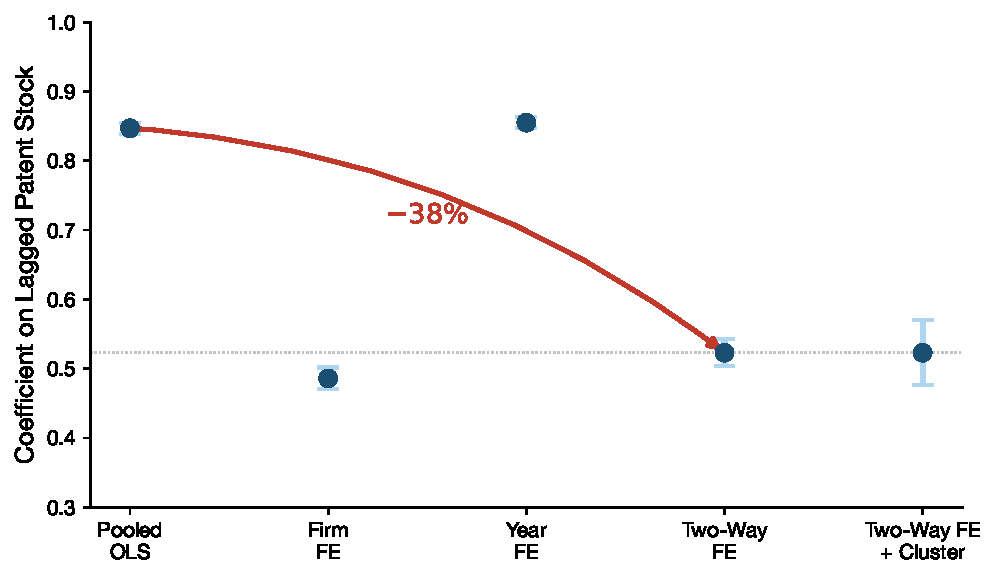
\includegraphics[width=\textwidth]{figures/coefficient_path.pdf}
\end{column}
\end{columns}
\end{frame}

% ──────────────────────────────────────────────────────────────────────────────
\begin{frame}{Large cross-sectional variation in innovation demands panel methods}

\vspace{0.3cm}

\textbf{Source:} Bena, Ortiz-Molina \& Simintzi (2022), ``Shielding Firm Value:
Employment Protection and Process Innovation,'' \textit{Journal of Financial Economics}.

\vspace{0.4cm}

\begin{table}
\centering\small
\begin{tabular}{@{}lrrrrr@{}}
\toprule
& \textbf{Mean} & \textbf{Std.\ Dev.} & \textbf{Min} & \textbf{Median} & \textbf{Max} \\
\midrule
Process innovation      & 1.137 & 1.824 & 0.000 & 0.000 & 10.100 \\
Product innovation      & 1.875 & 2.193 & 0.000 & 0.000 & 10.479 \\
Lagged patent stock     & 1.705 & 1.605 & 0.000 & 1.314 &  9.105 \\
State-year patents      & 1.671 & 0.682 & 0.000 & 1.712 &  4.664 \\
Total patent claims     & 146.2 & 835.1 & 0.000 & 4.000 & 59{,}923 \\
\bottomrule
\end{tabular}
\end{table}

\vspace{0.3cm}

\begin{columns}[T]
\begin{column}{0.32\textwidth}
\centering
\textbf{45,263}\\[2pt]
{\small firm-year obs.}
\end{column}
\begin{column}{0.32\textwidth}
\centering
\textbf{4,447}\\[2pt]
{\small unique firms}
\end{column}
\begin{column}{0.32\textwidth}
\centering
\textbf{1975--1997}\\[2pt]
{\small sample period}
\end{column}
\end{columns}
\end{frame}


% ━━━━━━━━━━━━━━━━━━━━━━━━━━━━━━━━━━━━━━━━━━━━━━━━━━━━━━━━━━━━━━━━━━━━━━━━━━━━
\section{Building the Specification}

% ──────────────────────────────────────────────────────────────────────────────
\begin{frame}{The same equation under four different assumptions}

\vspace{0.3cm}

\textbf{Pooled OLS} --- no fixed effects:
\[
  \text{ProcessInnovation}_{it} = \beta_0 + \beta_1 \, \text{PatentStock}_{i,t-1}
  + \beta_2 \, \text{StateYearPatents}_{it} + \varepsilon_{it}
\]

\vspace{0.3cm}

\textbf{Two-way fixed effects} --- firm $\alpha_i$ and year $\gamma_t$:
\[
  \text{ProcessInnovation}_{it} = \alert{\alpha_i} + \alert{\gamma_t}
  + \beta_1 \, \text{PatentStock}_{i,t-1}
  + \beta_2 \, \text{StateYearPatents}_{it} + \varepsilon_{it}
\]

\vspace{0.4cm}

\begin{columns}[T]
\begin{column}{0.46\textwidth}
\begin{block}{Stata}
\vspace{0.2em}
{\ttfamily\scriptsize\color{TextGrey}%
reghdfe cl\_pcs L1log1pspat\\
\hspace*{1em}logstyrpat,\\
\hspace*{1em}absorb(gvkey fyear)\\
\hspace*{1em}cluster(gvkey)}
\vspace{0.2em}
\end{block}
\end{column}
\begin{column}{0.46\textwidth}
\begin{block}{Python (pyfixest)}
\vspace{0.2em}
{\ttfamily\scriptsize\color{TextGrey}%
pf.feols(\\
\hspace*{1em}"cl\_pcs \texttildelow{} L1log1pspat\\
\hspace*{2em}+ logstyrpat | gvkey + fyear",\\
\hspace*{1em}data=df,\\
\hspace*{1em}vcov=\{"CRV1": "gvkey"\})}
\vspace{0.2em}
\end{block}
\end{column}
\end{columns}

\vspace{0.2cm}
{\scriptsize\color{MedGrey} Note: The original paper clusters by state (treatment level). Here we cluster by firm for illustration.}
\end{frame}


% ──────────────────────────────────────────────────────────────────────────────
\begin{frame}{Firm and year FE together isolate within-firm, within-year variation}

\vspace{0.3cm}

\begin{center}
\begin{tikzpicture}[
  box/.style={draw=DarkNavy, fill=LightGrey, rounded corners=4pt,
              minimum width=4.2cm, minimum height=1.6cm, align=center,
              font=\small},
  label/.style={font=\footnotesize\color{TextGrey}, align=center},
  arr/.style={-{Stealth[length=6pt]}, thick, DarkNavy},
  ]

  % Firm FE box
  \node[box] (firm) at (0,0) {%
    \textbf{Firm FE} ($\alpha_i$)\\[4pt]
    Industry, culture,\\
    location, management
  };

  % Year FE box
  \node[box] (year) at (6.5,0) {%
    \textbf{Year FE} ($\gamma_t$)\\[4pt]
    Recessions, patent law\\
    changes, tech shocks
  };

  % What remains
  \node[box, fill=white, draw=Accent, thick] (within) at (3.25,-3) {%
    \textbf{What identifies $\beta$}\\[4pt]
    Within-firm, within-year\\
    variation only
  };

  % Arrows
  \draw[arr] (firm.south) -- (within.north west);
  \draw[arr] (year.south) -- (within.north east);

  % Labels
  \node[label, above=0.15cm of firm] {absorbs time-invariant\\firm characteristics};
  \node[label, above=0.15cm of year] {absorbs common\\time shocks};

\end{tikzpicture}
\end{center}

\end{frame}


% ──────────────────────────────────────────────────────────────────────────────
\begin{frame}{Firm FE cuts the patent stock coefficient nearly in half}

\vspace{0.2cm}

\begin{table}
\centering\small
\begin{tabular}{@{}lccc@{}}
\toprule
& \textbf{(1) Pooled OLS} & \textbf{(2) Firm FE} & \textbf{(3) Year FE} \\
\midrule
Lagged patent stock
  & 0.847$^{***}$ & \alert{0.486$^{***}$} & 0.855$^{***}$ \\
  & \footnotesize(0.004) & \footnotesize(0.008) & \footnotesize(0.004) \\[6pt]
State-year patents
  & $-$0.019$^{*}$\phantom{**} & 0.312$^{***}$ & $-$0.069$^{***}$ \\
  & \footnotesize(0.008) & \footnotesize(0.019) & \footnotesize(0.008) \\
\midrule
Firm FE  & & $\checkmark$ & \\
Year FE  & & & $\checkmark$ \\
\midrule
$N$      & 45{,}263 & 44{,}898$^\dagger$ & 45{,}263 \\
$R^2$    & 0.555 & 0.745 & 0.569 \\
\bottomrule
\end{tabular}
\end{table}

\vspace{0.2cm}

Column (2): once we compare each firm \textit{to itself} over time, the
estimated effect of patent stock on process innovation
\alert{drops from 0.847 to 0.486} --- much of the pooled estimate
reflected persistent cross-firm differences, not a causal within-firm effect.

\vspace{0.15cm}
{\scriptsize $^\dagger$365 singleton firms (one observation only) are dropped when firm FE are included.}

\end{frame}


% ──────────────────────────────────────────────────────────────────────────────
\begin{frame}{Clustering doubles standard errors but does not change point estimates}

\vspace{0.2cm}

\begin{columns}[T]
\begin{column}{0.54\textwidth}

\begin{table}
\centering\footnotesize
\setlength{\tabcolsep}{3.5pt}
\begin{tabular}{@{}lcc@{}}
\toprule
& \textbf{(4) Two-Way FE} & \textbf{(5) Two-Way FE} \\
& \textbf{(IID SE)} & \textbf{(Clustered SE)} \\
\midrule
Patent stock
  & 0.523$^{***}$ & 0.523$^{***}$ \\
  & \scriptsize(0.010) & \scriptsize\alert{(0.024)} \\[6pt]
State-year pat.
  & 0.114$^{***}$ & 0.114$^{**}$\phantom{*} \\
  & \scriptsize(0.022) & \scriptsize\alert{(0.036)} \\
\midrule
Firm + Year FE  & $\checkmark$ & $\checkmark$ \\
S.E.\ type & IID & \alert{Clustered} \\
\midrule
$N$      & 44{,}898 & 44{,}898 \\
$R^2$    & 0.749 & 0.749 \\
\bottomrule
\end{tabular}
\end{table}

\end{column}
\begin{column}{0.42\textwidth}
  \centering
  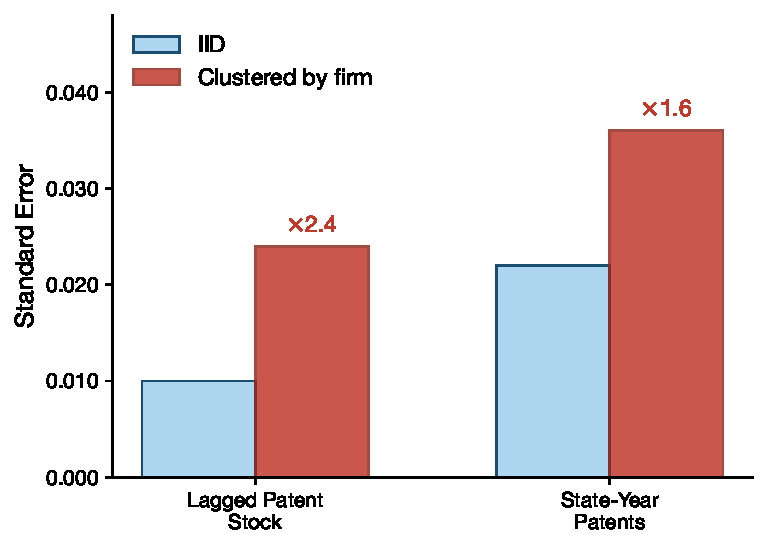
\includegraphics[width=\textwidth]{figures/se_comparison.pdf}

  \vspace{0.2cm}
  {\small IID SEs assume independence.
  Petersen (2009, \textit{RFS}) shows they
  are biased downward in panels.}

  \vspace{0.15cm}
  {\small\textbf{Rule:} Cluster at minimum by
  firm, or at the treatment level.}
\end{column}
\end{columns}

\end{frame}


% ━━━━━━━━━━━━━━━━━━━━━━━━━━━━━━━━━━━━━━━━━━━━━━━━━━━━━━━━━━━━━━━━━━━━━━━━━━━━
\section{Putting It Together}

% ──────────────────────────────────────────────────────────────────────────────
\begin{frame}{The coefficient halves, but remains significant across all specifications}

\vspace{0.2cm}

\begin{table}
\centering\footnotesize
\begin{tabular}{@{}lccccc@{}}
\toprule
& \textbf{(1)} & \textbf{(2)} & \textbf{(3)} & \textbf{(4)} & \textbf{(5)} \\
& Pooled OLS & Firm FE & Year FE & Two-Way FE & Two-Way FE \\
\midrule
Lagged patent stock
  & 0.847$^{***}$ & 0.486$^{***}$ & 0.855$^{***}$ & 0.523$^{***}$ & 0.523$^{***}$ \\
  & \scriptsize(0.004) & \scriptsize(0.008) & \scriptsize(0.004) & \scriptsize(0.010) & \scriptsize\alert{(0.024)} \\[4pt]
State-year patents
  & $-$0.019$^{*}$\phantom{**} & 0.312$^{***}$ & $-$0.069$^{***}$ & 0.114$^{***}$ & 0.114$^{**}$\phantom{*} \\
  & \scriptsize(0.008) & \scriptsize(0.019) & \scriptsize(0.008) & \scriptsize(0.022) & \scriptsize\alert{(0.036)} \\
\midrule
Firm FE  & & $\checkmark$ & & $\checkmark$ & $\checkmark$ \\
Year FE  & & & $\checkmark$ & $\checkmark$ & $\checkmark$ \\
S.E.\ type & IID & IID & IID & IID & Clustered \\
\midrule
$N$      & 45{,}263 & 44{,}898 & 45{,}263 & 44{,}898 & 44{,}898 \\
$R^2$    & 0.555 & 0.745 & 0.569 & 0.749 & 0.749 \\
\bottomrule
\end{tabular}
\end{table}

\vspace{0.2cm}
{\small Reading left to right: the pooled OLS estimate (0.847) is contaminated by
between-firm variation. Firm FE cuts it to 0.486. Adding year FE \textit{on
top of} firm FE raises the coefficient slightly to 0.523. Clustering doubles
the standard error but the effect remains significant at the 0.1\% level.}

\end{frame}


% ──────────────────────────────────────────────────────────────────────────────
\begin{frame}{Patent stock predicts both process and product innovation equally}

\vspace{0.4cm}

\begin{columns}[T]
\begin{column}{0.5\textwidth}

\begin{table}
\centering\small
\begin{tabular}{@{}lcc@{}}
\toprule
& \textbf{Process} & \textbf{Product} \\
\midrule
Lagged patent stock
  & 0.523$^{***}$ & 0.522$^{***}$ \\
  & \footnotesize(0.024) & \footnotesize(0.026) \\[6pt]
State-year patents
  & 0.114$^{**}$\phantom{*} & 0.136$^{**}$\phantom{*} \\
  & \footnotesize(0.036) & \footnotesize(0.042) \\
\midrule
Firm FE  & $\checkmark$ & $\checkmark$ \\
Year FE  & $\checkmark$ & $\checkmark$ \\
Clustered SE & $\checkmark$ & $\checkmark$ \\
\midrule
$N$      & 44{,}898 & 44{,}898 \\
$R^2$    & 0.749 & 0.718 \\
\bottomrule
\end{tabular}
\end{table}

\end{column}
\begin{column}{0.46\textwidth}
  \centering
  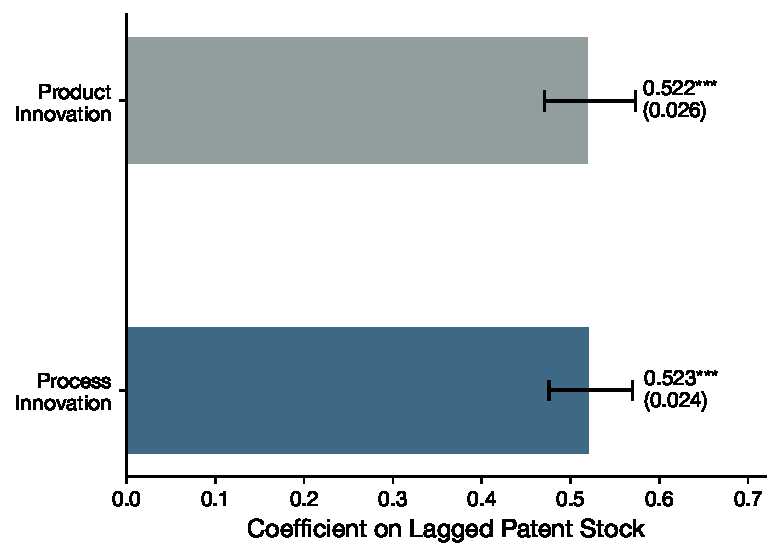
\includegraphics[width=\textwidth]{figures/process_vs_product.pdf}
\end{column}
\end{columns}

\vspace{0.1cm}
{\small The coefficient on patent stock is nearly identical for both outcomes.
The regional innovation environment matters slightly more for product innovation.}

\end{frame}


% ━━━━━━━━━━━━━━━━━━━━━━━━━━━━━━━━━━━━━━━━━━━━━━━━━━━━━━━━━━━━━━━━━━━━━━━━━━━━
\section{For Your Dissertation}

% ──────────────────────────────────────────────────────────────────────────────
\begin{frame}{Your dissertation regressions need these safeguards}

\vspace{0.4cm}

\begin{enumerate}
  \item \textbf{Always include fixed effects.}
        Pooled OLS produces biased estimates when unobserved
        heterogeneity correlates with regressors.

  \vspace{0.35cm}

  \item \textbf{Two-way FE (firm + year) is the standard.}
        Absorbs both persistent firm differences and aggregate
        time shocks.

  \vspace{0.35cm}

  \item \textbf{Always cluster standard errors.}
        At minimum by firm. At the treatment level if higher
        (state, industry).
\end{enumerate}

\end{frame}


% ──────────────────────────────────────────────────────────────────────────────
\begin{frame}{Show your readers the specification matters}

\vspace{0.4cm}

\begin{enumerate}
  \setcounter{enumi}{3}

  \item \textbf{Show multiple specifications.}
        Present pooled OLS $\rightarrow$ firm FE $\rightarrow$
        two-way FE to demonstrate robustness.

  \vspace{0.35cm}

  \item \textbf{Watch how coefficients change.}
        Large drops signal omitted variable bias in simpler models.

  \vspace{0.35cm}

  \item \textbf{Watch how standard errors change.}
        Clustering typically inflates SEs --- if it doesn't,
        question whether your panel has meaningful within-cluster
        correlation.
\end{enumerate}

\end{frame}


% ──────────────────────────────────────────────────────────────────────────────
\begin{frame}{Your coefficient tells a different story depending on what you absorb}

\vspace{1.2cm}

\begin{center}
\begin{tikzpicture}
  \node[font=\Large\bfseries, text=DarkNavy, text width=11cm, align=center] {%
    The same data.\\[6pt]
    The same regression.\\[6pt]
    The same variable.\\[12pt]
    \alert{$\hat{\beta} = 0.847$} \quad or \quad \alert{$\hat{\beta} = 0.523$}\\[12pt]
  };
  \node[font=\normalsize, text=TextGrey, text width=11cm, align=center] at (0,-2.3) {%
    Fixed effects don't change the data ---\\
    they change what variation identifies your estimate.
  };
\end{tikzpicture}
\end{center}

\end{frame}


% ──────────────────────────────────────────────────────────────────────────────
\begin{frame}{References}

\vspace{0.3cm}
\small

\textbf{Data source}

\vspace{0.15cm}

Bena, J., Ortiz-Molina, H. \& Simintzi, E. (2022). Shielding firm value:
Employment protection and process innovation. \textit{Journal of Financial
Economics}, 146(2), 637--664.

\vspace{0.5cm}

\textbf{Methodology}

\vspace{0.15cm}

Petersen, M.A. (2009). Estimating standard errors in finance panel data sets:
Comparing approaches. \textit{Review of Financial Studies}, 22(1), 435--480.

\vspace{0.15cm}

Breuer, M., Leuz, C. \& Vanhaverbeke, S. (2024). Using and interpreting
fixed effects models. \textit{Journal of Accounting Research}, 62(4).

\vspace{0.15cm}

Angrist, J.D. \& Pischke, J.-S. (2009). \textit{Mostly Harmless
Econometrics}, Chapter 5.

\end{frame}

\end{document}
